\documentclass[a4paper]{article}

%% Language and font encodings
\usepackage[english]{babel}
\usepackage[utf8x]{inputenc}
\usepackage[T1]{fontenc}

%% Sets page size and margins
\usepackage[a4paper,top=3cm,bottom=2cm,left=3cm,right=3cm,marginparwidth=1.75cm]{geometry}

%% Useful packages
\usepackage{amsmath}
\usepackage{amssymb}
\usepackage{graphicx}
\usepackage[colorinlistoftodos]{todonotes}
\usepackage[colorlinks=true, allcolors=blue]{hyperref}
\usepackage{times}
\usepackage{url}
\usepackage{latexsym}
\usepackage{natbib}
\usepackage{graphicx}
\usepackage{paralist}
\graphicspath{ {figs/} }


%% \usepackage[numbers]{natbib}

\title{Multi-task Learning for Event-Participant Embeddings}
\author{Author: Xudong Hong \\ 
Supervisor: Asad Sayeed, Vera Demberg}

\begin{document}
\maketitle

\begin{abstract}
\noindent
We introduce several neural network models to learn embeddings containing both lexical and semantic features of events and event participants. Possible methods to compose word and semantic role representations are discussed. Making use of tensor factorisation on role-specific word embedding \citep{tilk2016event}, we represent the order-3 tensor with three matrices. Then we add non-linearity and construct the model as a neural network. The model is trained in multitask style to perform both semantic role-filler prediction and semantic role prediction. Comparing to previous work, the model has improved on both semantic role/role-filler modelling and human thematic fit judgement correlations task. Moreover, the trained model has high accuracy on semantic role prediction. The high-level features of the model can be used in incremental semantic role labelling.  
\end{abstract}



\section{Introduction} \label{sec:intro}
In natural language understanding, the representation of events and their participants take an important role. To understand different sentences, we need to focus on event-level information among them  (see Section \ref{sec:event}). For example, in sentences like: 
\begin{eqnarray}
    & &\text{The cook cut the cake with knife in the kitchen.}        \label{eg:sent1} \\   
    & &\text{In the kitchen, the cake is cut with knife by the cook.} \label{eg:sent2}
\end{eqnarray}
the event-level information is actually the same. The event is described by the predicate $cut$ and the participants of this event are $cook$, $cake$, $knife$ and $kitchen$. Although the syntactic roles of participant $cook$ in two sentences are different (subject in sentence \eqref{eg:sent1} and object in sentence \eqref{eg:sent2}), they are both the $cutter$ of the $cake$. This shared information can be capture by a level of shallow semantic representation: \textit{semantic roles} \citep{jurafsky2014speech}. 

Semantic roles express the abstract roles of participant can taken in an event. In this level of representation, event participants can be mapped to arguments where they located. Using \textit{thematic role}, an inventory of conceptual argument roles (see Section \ref{sec:semanticrole}), the two sentences in earlier example can be annotated as: 
\begin{eqnarray} \label{eg:thematic}
  \nonumber & &[_{\text{AGENT}} \text{The }\textbf{cook}]\ cut\ [_{\text{PATIENT}}\text{the }\textbf{cake}]\ [_{\text{INSTRUMENT}}\text{with }\textbf{knife}]\\  
    & &[_{\text{LOCATION}}\text{in the }\textbf{kitchen}]. \\
  \nonumber & &[_{\text{LOCATION }}\text{In the }\textbf{kitchen}],\ [_{\text{PATIENT }}\text{the }\textbf{cake }]\ is \ cut\ \\
    & &[_{\text{INSTRUMENT }}\text{with }\textbf{knife}]\ [_{\text{AGENT }}\text{by the }\textbf{cook}]. 
\end{eqnarray} 
where the event participants are actually head nouns or noun-noun compounds inside arguments of the predicate $cut$. $The\ cook$, volitional causer of the event, has a AGENT role and $the\ cake$, the participant mostly affected by the event, has a PATIENT role. But it has been shown that it is hard to define thematic role formally. As a result, the PropBank \citep{palmer2005proposition} style semantic role model is introduced where each semantic role is associated with a specific verb sense. So the representation of two sentences can be unified as: 
\begin{equation*} \label{eg:probank}
\begin{aligned}
    & \text{Predicate: }&&cut.\textbf{01} \\
    & \text{Arguments: }&&[_{\text{ARG0 }}\text{The }\textbf{cook}], \ [_{\text{ARG1 }}\text{the }\textbf{cake}], \ [_{\text{ARGM-MNR }}\text{with a }\textbf{knife}], \\
    &           &&[_{\text{ARGM-LOC }}\text{in the }\textbf{kitchen}]
\end{aligned}
\end{equation*} 
where each argument is assigned with a semantic role label. $cut.01$ is the verbal predicate $cut$ with sense $01$ which is \textit{"make an incision or separation"}. Now the ARG0 role can be defined exactly as \textit{"the subject which makes incision"}. To obtain this representation from raw text, one needs to solve semantic role labelling task (see Section \ref{sec:srl}). 

Since both raw words and semantic role labels are symbols, it has limited representing power. If someone wants to compare events quantitatively, it is not possible to use the \textit{symbolic representation} where each symbol represent a single state of the entry. There are some previous works construct representation of linguistic units e.g. \textit{Distributional semantic model} (DSM) (see Section \ref{sec:dsm}). Amoung them, \textit{Distributed representation} of words, also named as \textit{word embedding}, is a well-established technique based on continuous feature space. Each word is represented by a low-dimensional dense vector with real number parameters, where those parameters are learnt during training of a prediction task given the context. There are many efforts on learning word embeddings from large scale corpora (see Section \ref{sec:repr}). 


\subsection{Main Problem and Previous Work}
The main problem is that only a few works learn embeddings of information inside events. \citet{tilk2016event} proposed two models trained to learn a representation of events and their participants. To obtain a probability distribution over role-fillers given the event information, the models aim to perform \textit{role-filler prediction}: In each event, given the role label of one target word, and also given all other words and their role labels, the task is to predict the target word to fill the target role. The predicate is considered as a special role label which is not in PropBank style semantic roles. The representation, named as \textit{role-specific word embedding}, learnt by those models is organised into an order-3 tensor. This means that for each word and each role, there is an embedding vector. They reported great improvement over previous systems on thematic fit evaluation and competitive performance on event similarity evaluation. However, the definition of notion \textit{role} is vague. It is hard to explain why predicates and semantic role-fillers are treated as the same. In addition to that, there is a problem of event embedding if we only focus on role-filler prediction. The event embeddings with same argument words but different roles can be very similar to each other. For example, the embedding vector of $([_\text{ARG0 }\text{boy}], [_\text{PREDICATE }\text{eat}], [_\text{ARG1 }\text{apple}])$ can be very similar to the embedding vector of $([_\text{ARG0 }\text{apple}], [_\text{PREDICATE }\text{eat}], [_\text{ARG1 }\text{boy}])$, where $cut$ is the shared predicate. 


\subsection{Major Tasks and Contribution}
In this paper, we present several multi-task neural network models to learn embeddings at the inner level of event. With a view to the explainability of the task, we separate \textit{role-filler prediction} into two sub-tasks: 
\begin{itemize}
  \item  \textbf{Participant prediction}: in each event, given the predicate, the semantic role label of one target participant, the other participants and their semantic role labels, the task is to predict the target participant to fill the semantic role. 
  \item  \textbf{Predicate prediction}: in each event, given all participants and their semantic role labels, the task is to predict the predicate. 
\end{itemize}
where participant and predicate can be combined as \textit{role-filler}. Since their lexical features are homogeneous, we can consider each role-filler as a word. To get rid of ambiguity, we define \textbf{semantic role labels} as a set which contains semantic role labels in PropBank style for event participants and a special semantic role label PREDICATE for predicates. In order to tackle the similarity problem in event embedding stated above, we add one more auxiliary task which is: 
\begin{itemize}
  \item  \textbf{Semantic role label prediction}: in each event, given one target word, and all other words and their semantic role labels, the task is to predict the target semantic role label. 
\end{itemize}
By forcing the models to solve semantic role label prediction during training, the event embeddings with same words but different roles will be distinguished. 

Inspired by the role-specific word embedding, we define the \textbf{event-participant embedding} formally as the joint embedding of predicates that denote events and participants of events. The embedding vectors are stacked together to construct an order-3 tensor where each vector is indexed by a 2-tuple $(word, role\ label)$. As a result, each word can be represented as a matrix, indexed by an 1-tuple $(word)$, which can be easily reshaped into a word embedding vector (see Section \ref{sec:epe}). Although the event-participant embedding is a versatile representation, it suffers the curse of dimensionality. So we apply tensor factorisation on the event-participant embedding tensor, which factorise the tensor into three matrices. After detailed analysis in the tensor space, we demonstrate that these matrices can be interpreted as word embedding, semantic role label embedding and projection weight correspondingly (see Section \ref{sec:tf}). 

Using the same event-participant embedding as input, we add non-linearity to the models to construct multitask neural networks. To perform both role-filler prediction and semantic role label prediction, we design two classifiers with their own loss functions. The models are optimised with different weight of each task (see Section \ref{sec:mtl}). We find that tuning the loss weight results in models having their own advantages in different aspects. When it comes to the construction of event representation, there are two cases: word order is known and unknown. In this paper, we focus on the case which word order is not given. After comparing several composition methods, we present an effective method to compose the event-level embedding using features from hidden layer (see Section \ref{sec:composition}). It has been shown that gradient exploding or vanishing problem is more serious in training model with factorised tensors \citep{sutskever2011generating}.  Making use of the idea in residual learning, we add one skip connection inside the factor tensor (see Section \ref{sec:residual}). We find that this method can help with learning a better event-participant embedding.

To compare with previous baselines, all models are trained, validated and tested on the same corpus. Hyper-parameters are tuned to optimise for different purposes (see Section \ref{sec:exp}). The output probabilities of the models on word prediction are evaluated on human thematic fit judgement correlation task (see Section \ref{sec:thematicfit}). The word embeddings are evaluated on several word similarity tasks (see Section \ref{sec:wordsim}). Last but not least, the event embeddings are evaluated on a event similarity correlation task (see Section \ref{sec:eventsim}). The results show that our models has significant improvement over the current best system on specific evaluations while has state-of-the-art performance on the other evaluations. The word embedding and event embedding extracted from the event-participant embedding we learnt also has state-of-the-art performance. 

Our model is a state-of-the-art system in selectional preference task. The selectional preference features are useful for referent prediction in discourse level \citep{modi2017modeling}. The word embedding we learn can be further employed in discourse relation classification, paraphrase detection, word sense disambiguation, sentiment analysis and machine translation. The composite features of predicate and target semantic role label can be used for argument classification in semantic role labelling \citep{roth2016neural}. 



\section{Background}

\begin{table}[t]
\centering
\begin{tabular}{l|l}
\textbf{Thematic Role}  &   \textbf{Definition} \\ \hline
AGENT                   &   The volitional causer of an event \\
PATIENT (THEME)         &   The participant most directly affected by an event \\
INSTRUMENT              &   The inanimate force or object used in an event \\
LOCATION                &   The location or spatial orientation of the event \\
\end{tabular}
\caption{\label{tab:thematic} Definitions of common thematic roles.}
\end{table}


\subsection{Event Knowledge and Representation} \label{sec:event}
In psycholinguistics and cognitive science, experiments have shown that event knowledge plays a crucial role in human sentence processing \citep{camblin2007interplay}. On one hand, predicates prime event participant referring to good fillers of their semantic role in an event \citep{ferretti2001integrating}. On the other hand, priming effect can be also found from event participants to predicates \citep{mcrae2005basis}. These two works reveal that model performances of predicate prediction and participant prediction can be evaluated via correlation with human judgement. In a wider range, event-level information affects verbal arguments processing of human \citep{bicknell2010effects}. Comprehenders integrate information not only from predicate but also other event participants mentioned in discourse. Overall, it is necessary to obtain representation of events from sentences. 

In early research, events were represented using first order logic. For the event in the example sentence (\ref{eg:sent1}), the representation is:
\begin{equation*} \label{eg:fol}
\begin{aligned}
    & cut(\text{cook}, \text{cake}) \land with(\text{knife}) \land in(\text{kitchen}) \\
\end{aligned}
\end{equation*}
where it is hard to refer to predicates. Later on, \citet{davidson1967logical} proposed a method that linguistic predicates consider an event as one of their logical arguments explicitly. So the representation of the sentence (\ref{eg:sent1}) becomes: 
\begin{equation*} \label{eg:davidsonian}
\begin{aligned}
    & \exists e\ cut(e, \text{cook}, \text{cake}) \land with(e, \text{knife}) \land in(e, \text{kitchen}) \\
\end{aligned}
\end{equation*}
where the predicate $cut$ is a description of an event $e$. This representation, named as \textit{Davidsonian event representation}, has a drawback that it is hard to distinguish the roles of $cook$ and $cake$. Combining with thematic roles mentioned in session \ref{sec:intro}, \citet{parsons1990events} updated the representation to: 
\begin{equation*} \label{eg:neodavidsonian}
\begin{aligned}
    \exists e\ cut(e)
    & \land \text{AGENT}(e, \text{cook}) \land \text{PATIENT}(e, \text{cake}) \\
    & \land \text{INSTRUMENT}(e, \text{knife}) \land \text{LOCATION}(e, \text{kitchen}) \\
\end{aligned}
\end{equation*}
where each thematic role is acting as a logical predicate of the event $e$ and the corresponding participant. This representation, named as \textit{neo-Davidsonian event representation}, is highly compatible with semantic role models. 


\subsection{Semantic Role Models} \label{sec:semanticrole}
Thematic role is the oldest semantic role model which is formalised by \citet{gruber1965studies} and \citet{fillmore1968case} in modern time. The inventory of roles usually contains AGENT, PATIENT, INSTRUMENT and LOCATION \citep{aarts2013english}. Table \ref{tab:thematic} shows informal definitions of them \citep{jurafsky2014speech}. One disadvantage of thematic role is that the range of role inventory is difficult to decide. Even worse, the formal definitions of thematic roles are controversial. 

The Proposition Bank (PropBank) is an annotated corpus of semantic roles based on Penn TreeBank \citep{palmer2005proposition}. It also provides an effective semantic role model which we will adopt. Table \ref{tab:semantic} shows definitions of semantic roles in PropBank style used in this paper. The definitions are based on the PropBank Annotation Guidelines \citep{bonial2010propbank} except that the notion of argument is replaced by event participant. Arguments required for the valency of a predicate are listed with numbers. Modifiers, which are relatively stable across predicates, are marked with ArgMs. While PropBank focuses on verbal predicate, NomBank adds annotations to nominal predicates \citep{meyers2004nombank}. 


\begin{table}[t]
\centering
\begin{tabular}{l|l} 
\hline
\textbf{PropBank Semantic Role}  &   \textbf{Definition} \\ \hline
Arg0                    &   proto-agent, the argument that most likely to be the agent, \\ 
                        &   volitional causer or experiencer \\ \hline
Arg1                    &   proto-patient, the argument that most likely to be the patient \\ \hline
Arg2                    &   the instrument, benefactive or attribute \\ \hline
Arg3                    &   the starting point, benefactive or attribute \\ \hline
Arg4                    &   the ending point \\ \hline
ArgM-LOC                &   the argument that indicates where the action takes place \\ \hline
ArgM-MNR                &   the argument that specifies how the action is performed \\ \hline
ArgM-TMP                &   the argument that shows when an action took place \\ \hline
ArgM-PNC                &   the argument that shows motivation for some action \\ \hline
ArgM-CAU                &   the argument that indicates the reason for an action \\ \hline
\end{tabular}
\caption{\label{tab:propbank} Definitions of major semantic roles in PropBank style.}
\end{table}


\subsection{Semantic Role Labelling} \label{sec:srl}
The \textit{semantic role labelling} (SRL) task is to assign semantic role labels to arguments of predicates in sentences automatically. It is a well-study task which was defined formally at CoNLL 2004, 2005 shared tasks which aimed to annotate phrasal arguments of verbal predicates in the sentences \citep{carreras-marquez:2004:CONLL, carreras-marquez:2005:CoNLL}. The CoNLL 2008, 2009 shared tasks introduced a new task where the semantic dependencies are annotated instead of phrasal arguments \citep{surdeanu-EtAl:2008:CONLL, hajivc-EtAl:2009:CoNLL-2009-ST}. 

After many years of research, pre-trained semantic role labelling systems are quite reliable. Generally speaking, modern SRL system is a statistical model that can predict the semantic role labels given the sentences. Many early work used syntactic parses as input and estimate classifiers locally with a set of constraints \citep{punyakanok2008importance}. \citet{tackstrom2015efficient} interpreted the model as a graphical model and use multi-layer neural network to enforce the constraints. Later work focus on application of distributed representation to avoid feature engineering and result in better generalisation. \citet{collobert2007fast, collobert2011natural} proposed a convolution neural network model using distributed representation that only rely on lexical features. The fine-tuned model with additional features, SENNA, has state-of-the-art performance. The running time of SENNA is fast so it can be used on large corpus. 

More recently, \citet{lei-EtAl:2015:NAACL-HLT} employ low-rank tensor factorisation to induce a compact representation of the full cross product of atomic features. \citet{roth2016neural} proposed PathLSTM which made use of dependency path as input. \citet{marcheggiani2017simple} claimed that syntactic features is not necessary for semantic role labelling and proposed a deep LSTM model to obtain competitive performance. 


\subsection{Distributional Semantic Model} \label{sec:dsm}
Distributional semantic model (DSM) is a corpus-based method to construct numerical semantic representation. DSM depends on distributional hypothesis \citep{harris1954distributional, miller1991contextual} claiming that the semantic similarity between two linguistic units can be measured by the overlap among their contexts. A DSM can be viewed as an order-2 tensor where one dimension is index of word (or lexical unit) and another dimension is the feature that used to capture context information. Generally in early work of DSM, a matrix was constructed based on lexical co-occurrences of words in a large corpus. Then each word can be represented by a high-dimensional sparse vector in this matrix. The semantic similarity between two units can be quantified as the similarity of two representation vectors. This however does not consider the linguistic information within the context. To include such information, later work encode syntactic relation or lexico-syntactic pattern \citep{pado2007integration, erk2008structured, rothenhausler2009unsupervised} (performance?). 

\citet{baroni2010distributional} claimed that it is possible to construct a general model for semantic memory, a stable long-term knowledge of human, to tackle different semantic tasks. They proposed \textit{Distributional Memory} (DM) framework which is an order-3 tensor which contains word-relation-word tuple. Performing matricisation on the tensor onto a matrix, vectors from different semantic spaces can be obtained. On tasks of a broad range, their best model, named as TypeDM, obtained state-of-the-art performance. This can be interpreted as the advantage of the distributional representation on multiple semantic tasks. Furthermore, the tensor like structure is both flexible and expressive for semantic information modelling. 

In addition to syntactic information, \citet{sayeed2014combining} extracts shallow semantic representation using semantic role labeller SENNA and constructs DM upon them. Combining syntactic and semantic features, they build a fully unsupervised distributional memory model, named as SDDM, especially for thematic fit judgement task. SDDM outperforms syntax-based thematic fit model by a large margin, which indicates that semantic information is essential in thematic fit task. 

There are three major drawbacks of distributional semantic model. Firstly when it comes to practice, the semantic space of DSM is high-dimensional and sparse. When someone wants to induce on complex events with large number of participants, using sparse vectors is unfeasible. In addition, the parameters of the vectors is discrete in count-based vector space. Although many alternative weighting functions and smoothing techniques has been proposed, it is hard to decide which is the most optimised. Last but not least, these models usually suffer curse of dimensionality. Because the Euclidean distance between two vectors is meaningless in high-dimensional space, when the representation vectors are used as input of distance-based algorithms like nearest-neighbour classifier or clustering, the result can be unexpected. Thus we need a better representation model in this paper. 

\subsection{Distributed Representation} \label{sec:repr}
Distributed representation, pioneered by \citet{hinton1986learning}, is an effective method to handle sparsity and curse of dimensionality in symbolic representation. In general symbolic representation like \textit{one-hot representation}, where one binary value is $1$ and the others are $0$ in representation vectors, the binary values are mutual exclusive. If each representation vector has $n$ features, it can only represent $n$ different states of the entry. In distributed representation, $n$ feature with $k$ possible values can describe $k^n$ different states \citep{Goodfellow-et-al-2016}. This is why distributed representation is powerful. 

The distributed representation of words, popularly known as word embedding, can be learnt in the training of \textit{neural net language model} \citep{bengio2003neural}. Most of early work aimed to solve language modelling which is the task to predict the target word given its context. Unlike DSMs or other count-based semantic models, the parameters in distributed representation vectors are learnt during the training of neural net language models. Later these models were further improved by making use of sequential information in previous context of target words. This can be done by adding recurrent units to hidden layers of neural net language model \citep{mikolov2010recurrent}. To learn high quality word embeddings with million words in the vocabulary from a billion scale of text, \citet{mikolov2013efficient} proposed two models, \textit{CBOW} and \textit{Skip-gram}, based on logistic regression. Context is the words around the target word in both models. In CBOW model, context representation is the sum of word embedding vectors of the words in the context. In Skip-gram model, the target word is used to predict the words in the context. The system they built, famously known as \textit{word2vec}, obtained competitive performance against more complex neural networks on syntactic and semantic relation tasks. To tackle multiple tasks in natural language processing, \citet{collobert2011natural} proposed a model which shares the word embedding across tasks of language modelling, part-of-speech tagging, chunking, named entity recognition, semantic role labelling. 


\section{Representation of Predicates and Participants}
\subsection{Event-Participant Embedding} \label{sec:epe}
We intend to learn meaningful representation of event structure in semantic space. Firstly we define the symbolic representation for words. Word $a_i$ is encoded as one-hot row vector $\mathbf{w}_i$ where $|\mathbf{w}_i| = |V|$ and $V$ is the word vocabulary. In this vector space, words are mutual exclusive to each other. Similarly, we can represent semantic role label $b_j$ using one-hot encoded column vector $\mathbf{r}_j$ where $|\mathbf{r}_j| = |R|$ and $R$ is the set of semantic role labels including semantic roles and a special role PREDICATE. 

Further than that, we need to obtain a distributed representation that is continuous in the feature space. So we compute the inner product between $\mathbf{w}_i$ and a embedding matrix $\mathbf{A} \in \mathbb{R}^{|V| \times k}$ as $\mathbf{A}_{(i)} = \mathbf{w}_i \mathbf{A}$. The vector $\mathbf{w}_i$ is now mapped to low-dimensional vector $\mathbf{A}_{(i)} \in \mathbb{R}^k$ which is the $i$-th row of matrix $\mathbf{A}$. The symbolic representation of words is transformed into word embedding. 

In addition to word embedding, we want to learn the representation of words given a specific semantic role label. We add one more dimension of semantic role label to the word embedding matrix and obtain a third-order tensor $\mathbf{T} \in \mathbb{R}^{|V| \times |R| \times d}$. For each word $\mathbf{w}_i$ and each semantic role label $\mathbf{r}_j$, there is a corresponding vector $\mathbf{T}_{(ij)}$ with length of $d$ where $i \in [1, |V|]$ and $j \in [1, |R|]$. We define this vector as \textbf{event-participant embedding vector}. 


\subsection{Tensor Factorisation} \label{sec:tf}
There are $|V| \times |R| \times d$ parameters in the order-3 tensor $\mathbf{T}$. Since word vocabulary size $|V|$ is often very big (more than $50,000$), the number of parameters in the tensor grows tremendously when $|R|$ or $d$ increases, which makes the model hard to converge. The huge number of parameters in event-participant embedding can result in curse of dimensionality. Moreover, \citep{tilk2016event} pointed out that this kind of embedding tensor lacks parameter sharing across word embedding matrices between different role labels, while words with the same semantic role label actually have common characteristics. In order to capture these characteristics, we need a method to share weights between word embedding matrices. 

We perform tensor rank decomposition \citep{hitchcock1927expression} on the embedding tensor in real space:
\begin{equation} \label{eq:trd_org}
\begin{aligned}
    \mathbf{T}   
        &= \sum_{m=1}^{k} \lambda_m \mathbf{T}'_m \\
        &= \sum_{m=1}^{k} \lambda_m \mathbf{a}_m \otimes \mathbf{b}_m \otimes \mathbf{d}_m, \\
\end{aligned}
\end{equation}
where tensor $\mathbf{T}$ is decomposed into $k$ rank-1 tensor $\mathbf{T}'$ and $\lambda_m$ is the weight of rank $m$. Each rank-1 tensor can be written as outer product of 3 row vectors $\mathbf{a}_m$, $\mathbf{b}_m$ and $\mathbf{d}_m$. Since all parameters are learnt during training, we let $\mathbf{c}_m$ equal to $\lambda_m \mathbf{d}_m$. So the equation becomes:
\begin{equation} \label{eq:trd}
\begin{aligned}
    \mathbf{T}   
        &= \sum_{m=1}^{k} \mathbf{a}_m \otimes \mathbf{b}_m \otimes \mathbf{c}_m, \\
\end{aligned}
\end{equation}
where the smallest $k$ makes the equation true is the tensor rank of $\mathbf{T}$. Now the number of parameters is reduced to $(|V| + |R| + d) \times k$ which is comparable smaller. 


\subsection{Interpretation of Factored Tensor} \label{sec:tf-expl}
We then group $k$ vectors $\mathbf{a}_m$, $\mathbf{b}_m$ by column into matrices $\mathbf{A} \in \mathbb{R}^{|V| \times k}$, $\mathbf{B} \in \mathbb{R}^{|R| \times k}$ and $\mathbf{c}_m$ by row into matrices $\mathbf{C} \in \mathbb{R}^{k \times d}$. 

[TODO: formal interpretation] Naturally, matrix $\mathbf{A}$ can be interpreted as word embedding described above. $\mathbf{B}$ can be considered as role embedding matrix. By computing inner product between $\mathbf{r}_j$ and $\mathbf{B}$ as $\mathbf{B}_{(j)} = \mathbf{r}_j \mathbf{B}$, we obtain the low-dimensional vector $\mathbf{B}_{(j)} \in \mathbb{R}^k$ which is the $j$-th row of matrix $\mathbf{B}$. 

From equation \eqref{eq:trd}, the event-participant embedding vector $\mathbf{T}_{(ij)}$ can be computed as: 
\begin{equation} \label{eq:rbwe_tensor}
\begin{aligned}
    \mathbf{T}_{(ij)}
        &= \sum_{m=1}^{k} \mathbf{a}_{m_{(i)}} \otimes \mathbf{b}_{m_{(j)}} \otimes \mathbf{c}_m \\
        &= \sum_{m=1}^{k} \mathbf{a}_{m_{(i)}} \mathbf{b}_{m_{(j)}}  \mathbf{c}_m \\
\end{aligned}
\end{equation}
To get rid of the outer product and make it easier to implement, we use the decomposition matrices defined above. Thus the vector $\mathbf{T}_{(ij)}$ can be written as a vector: 
\begin{equation} \label{eq:rbwe}
\begin{aligned}
    \mathbf{p} 
        &= (\mathbf{A}_{(i)}\circ \mathbf{B}_{(j)}) \mathbf{C} \\
        &= (\mathbf{w}_i \mathbf{A} \circ \mathbf{r}_j \mathbf{B}) \mathbf{C} \\
\end{aligned}
\end{equation}
which is a representation of a participant in an event. "$\circ$" is Hadamard product which computes element-wise multiplication between two vectors. This can be interpreted as the composition method of word embedding vector and role embedding vector. 


\begin{figure}[t]
\centering
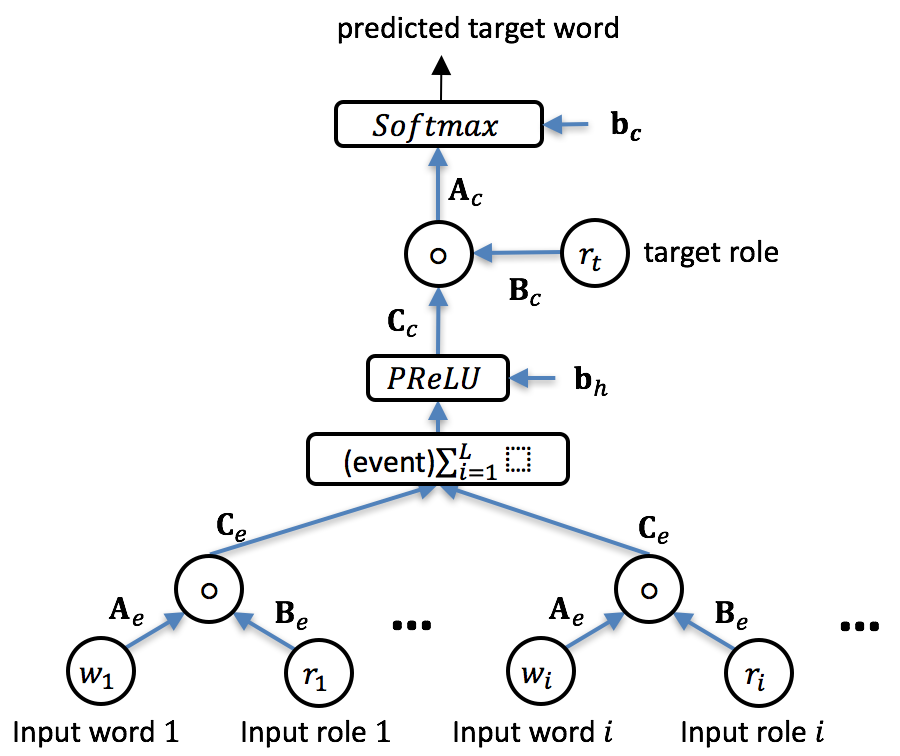
\includegraphics[width=0.65\textwidth]{NNRF.png}
\caption{\label{fig:NNRF} Model architecture of non-incremental role filler.}
\end{figure}


\section{Model Design}
\subsection{Non-incremental Role Filler} \label{sec:nnrf}
To perform the role-filler prediction, \citet{tilk2016event} proposed the \textit{non-incremental role filler} \textbf{(NNRF)} which is a 2-layer neural network model. As in Figure \ref{fig:NNRF}, from input to output, the model uses event-participant embeddings as input. Parameters are learnt together with the model. The embedding vector of the $l$-th entry in an event can be represented as:
\begin{equation} \label{eq:rbe_nnrf}
\begin{aligned}
    \mathbf{p}_l
        &= (\mathbf{w}_i \mathbf{A}_e \circ \mathbf{r}_j \mathbf{B}_e) \mathbf{C}_e \\
\end{aligned}
\end{equation}
The embedding vectors are composed using sum method into an representation of words except the target word as:
\begin{equation} \label{eq:sum_comp}
\begin{aligned}
    \mathbf{e}
        &= \sum_{l=1}^{L} \mathbf{p}_{l} \\
\end{aligned}
\end{equation}
where $l$ is the index of the participant and $L$ is the number of participants in current event $e$. Then it passes through one non-linearity layer with parametric rectified linear unit \citep{he2015delving} as follow:
\begin{equation} \label{eq:nonlinearity_nnrf}
\begin{aligned}
    \mathbf{h}
        &= PReLU(\mathbf{e} + \mathbf{b}_e) \\
\end{aligned}
\end{equation}
where $\mathbf{b}_e$ is the bias vector of this layer. After that, a softmax regression classifier is used for prediction. The output vector of this classifier is computed as:
\begin{equation} \label{eq:output_nnrf}
\begin{aligned}
    \mathbf{o}
        &= \mathbf{h}\mathbf{W}_c + \mathbf{b}_c \\
\end{aligned}
\end{equation}
where $\mathbf{W}_c\in \mathbb{R}^{d \times |V|}$ is a weight matrix of the target word classifier and $\mathbf{b}_c$ is the corresponding bias. The conditional probability of target word $a_x$ given event $e$ and target role $b_y$ is:
\begin{equation} \label{eq:softmax_nnrf}
\begin{aligned}
    p(a_x | e, b_y)
        &= Softmax(\mathbf{o})_{(x)} \\
        &= \frac{
        exp(\mathbf{o})_{(x)}
        }{
        \sum_{i=1}^{|V|} exp(\mathbf{o})_{(i)} }   \\
\end{aligned}
\end{equation}
where suffix $(x)$ is the $x$-th element of the vector. 

For each target target role, there is a different weight matrix to perform classification. \citet{tilk2016event} performed a similar technique like the role-specific word embedding. At first weight matrix $\mathbf{W}_c^{(b_y)}$ is defined for each target role $b_y$. Then those matrices $\mathbf{W}_c^{(b_y)}$ are stacked from $b_1$ to $b_{|R|}$. A weight tensor $\mathbf{T}^{(c)} \in \mathbb{R}^{d \times |R| \times |V|}$ is obtained. But this tensor suffer the same dimensionality problem as event-participant embedding tensor. So tensor rank decomposition is applied again on the weight tensor, and extract the corresponding weight matrices for $b_y$ as follow: 
\begin{equation} \label{eq:trd_cls}
\begin{aligned}
    \mathbf{T}_{(y)}^{(c)}
        &= \sum_{m=1}^{k^{(c)}} \mathbf{c}_{m}^{(c)} \otimes \mathbf{b}_{m_{(y)}}^{(c)} \otimes \mathbf{a}_m^{(c)} \\
\end{aligned}
\end{equation}
Similarly, vectors $\mathbf{c}_{m}^{(c)}$ are grouped by row into matrices $\mathbf{C}_c \in \mathbb{R}^{d \times k^{(c)}}$ and $\mathbf{a}_m^{(c)}$ are grouped by column into matrices $\mathbf{A}_c \in \mathbb{R}^{k^{(c)} \times |V|}$. After getting rid of outer product using same transformation as equation \eqref{eq:rbwe}, the weight matrix in equation \eqref{eq:output_nnrf}  can be written as:
\begin{equation} \label{eq:cls}
\begin{aligned}
    \mathbf{W}_c
        &= \mathbf{C}_c \ diag(\mathbf{b}_y) \ \mathbf{A}_c \\
\end{aligned}
\end{equation}
Since there is a vector $\mathbf{b}_y$ representing target role $b_y$, the embedding matrices $\mathbf{B}_c \in \mathbb{R}^{k^{(c)} \times |R|}$ can be defined for target roles. The weight matrices can be further written as:
\begin{equation} \label{eq:cls_temb}
\begin{aligned}
    \mathbf{W}_c
        &= \mathbf{C}_c \ diag(\mathbf{r}_y \mathbf{B}_c) \ \mathbf{A}_c \\
\end{aligned}
\end{equation}


\begin{figure}[t]
\centering
\includegraphics[width=0.7\textwidth]{MTNNRF.png}
\caption{\label{fig:MTNNRF} Model architecture of multitask version of non-incremental role filler.}
\end{figure}


For each target target role, there is a different weight matrix to perform classification. \citet{tilk2016event} performed a similar technique like the role-specific word embedding. At first weight matrix $\mathbf{W}_c^{(b_y)}$ is defined for each target role $b_y$. Then those matrices $\mathbf{W}_c^{(b_y)}$ are stacked from $b_1$ to $b_{|R|}$. A weight tensor $\mathbf{T}^{(c)} \in \mathbb{R}^{d \times |R| \times |V|}$ is obtained. But this tensor suffer the same dimensionality problem as event-participant embedding tensor. So tensor rank decomposition is applied again on the weight tensor, and extract the corresponding weight matrices for $b_y$ as follow: 
\begin{equation} \label{eq:trd_cls}
\begin{aligned}
    \mathbf{T}_{(y)}^{(c)}
        &= \sum_{m=1}^{k^{(c)}} \mathbf{c}_{m}^{(c)} \otimes \mathbf{b}_{m_{(y)}}^{(c)} \otimes \mathbf{a}_m^{(c)} \\
\end{aligned}
\end{equation}
Similarly, vectors $\mathbf{c}_{m}^{(c)}$ are grouped by row into matrices $\mathbf{C}_c \in \mathbb{R}^{d \times k^{(c)}}$ and $\mathbf{a}_m^{(c)}$ are grouped by column into matrices $\mathbf{A}_c \in \mathbb{R}^{k^{(c)} \times |V|}$. After getting rid of outer product using same transformation as equation \eqref{eq:rbwe}, the weight matrix in equation \eqref{eq:output}  can be written as:
\begin{equation} \label{eq:cls}
\begin{aligned}
    \mathbf{W}_c
        &= \mathbf{C}_c \ diag(\mathbf{b}_y) \ \mathbf{A}_c \\
\end{aligned}
\end{equation}
where $diag(\mathbf{v})$ is a diagonal matrix with vector $\mathbf{v}$ on its diagonal. Since there is a vector $\mathbf{b}_y$ representing target role $b_y$, the embedding matrices $\mathbf{B}_c \in \mathbb{R}^{k^{(c)} \times |R|}$ can be defined for target roles. The weight matrices can be further written as:
\begin{equation} \label{eq:cls_temb}
\begin{aligned}
    \mathbf{W}_c
        &= \mathbf{C}_c \ diag(\mathbf{r}_y \mathbf{B}_c) \ \mathbf{A}_c \\
\end{aligned}
\end{equation}



\section{Bag-of-Event-Participant Model} \label{sec:bop}

\begin{figure}[t]
\centering
\includegraphics[width=0.7\textwidth]{MTNNRF.png}
\caption{\label{fig:MTNNRF} Model architecture of multitask version of non-incremental role filler.}
\end{figure}


\subsection{Composition Method for Event Embedding} \label{sec:composition}
In the NNRF model, embedding vectors of event participants are sum up together to represent the whole event. Nonetheless, this is only a simple method to composite event participants. Each participant has same weight in the event. Additionally, means of parameters can shift in a large range the after the sum operation. How can we improve this? We need an exploration of composition methods. 

We separate all possible methods in two groups. The first group is \textbf{non-parametric methods} which have no extra parameters like addition, multiplication and concatenation of event participant vectors. Another group is \textbf{parametric methods} which need more parameters like recursive unit \citep{socher2013recursive}, recurrent unit \citet{mikolov2010recurrent}, or long-short-term-memory recurrent unit \citep{hochreiter1997LSTM}. So the NNRF is classified as non-parametric composition method. 

The second model proposed by \citet{tilk2016event}, \textit{incremental model}, is a parametric method. A recurrent unit is added to express participant order not only within event but also across different events. Moreover, a binary indicator $b$ is used to detect the event boundaries. $b$ equals to $1$ if the target word belongs to current event, otherwise $0$. So the event embedding vector is: 
\begin{equation} \label{eq:incremental}
\begin{aligned}
    \mathbf{e} 
        &= \mathbf{p} + \mathbf{h_{t-1}}\mathbf{W}_h + b\mathbf{v}, 
\end{aligned}
\end{equation}
where $\mathbf{v}$ is the parameter vector of event boundary. $\mathbf{h_{t-1}}$ is the hidden vector of last time step in the recurrent unit. $\mathbf{W}_h$ is the parameter matrix of recurrent unit. 

In this work, we focus on non-parametric methods in the condition that participant order is not provided and leave the other for future exploration. Multiplication is an effective composition method for distributed memory models. Unfortunately, during optimisation of neural network models, multiplication often results in extreme values which will lead to overflow or underflow. Concatenation is widely used in language modelling. But usually the concatenated feature can not be used directly. An extra feature extractor is needed, which turns it into a parametric method. 

We propose the \textbf{mean} composition method which compute the mean of all the  vectors of event participants to represent the event as one vector. Computing mean instead of sum can be considered as normalisation of participant representations within the event boundary, which can prevent possible overflow/underflow of the weights of hidden vector. 

Since it is a non-parametric method, we also want to add a weight before the mean composition. Instead of using a fully-connected layer, we apply the PReLU to each embedding vector of participant to obtain the hidden vector: 
\begin{equation} \label{eq:nonlinearity_bop}
\begin{aligned}
    \mathbf{h}_l
        &= PReLU_l(\mathbf{p}_l) \\
\end{aligned}
\end{equation}
So the parameters inside PReLU can also act as weights of each participant. Using the mean method, the embedding vectors are composed as:
\begin{equation} \label{eq:mean_comp_bop}
\begin{aligned}
    \mathbf{e}
        &= \frac{1}{L} \sum_{l=1}^{L} \mathbf{h}_{l} \\
\end{aligned}
\end{equation}
whehe $\frac{1}{L}$ is used to compute the empirical mean of the hidden vector. This model is named as \textbf{bag-of-event-participants (BOP)} described in Figure \ref{fig:BOP}. 


\begin{figure}[t]
\centering
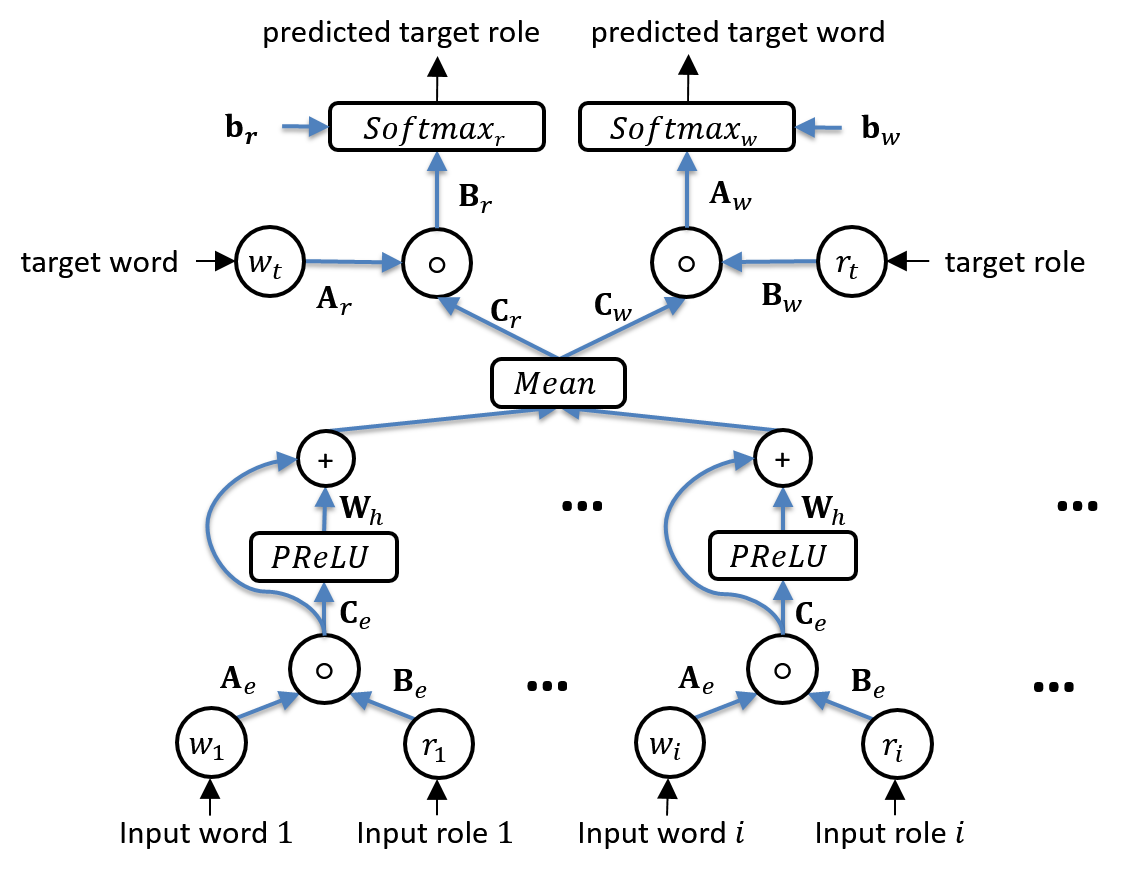
\includegraphics[width=0.8\textwidth]{BOPRes.png}
\caption{\label{fig:BOPRes} Model architecture of bag-of-event-participants with skip connection.}
\end{figure}


\subsection{Residual Learning} \label{sec:residual}


\newpage

\section{Experiments}  \label{sec:exp}
\subsection{Corpus and Prepossessing} \label{sec:corpus}







\section{Evaluation}  \label{sec:evaluation}
\subsection{Human Thematic Fit Judgement Correlation Task}  \label{sec:thematicfit}
To improve performance of DM on thematic fit task, \citet{greenberg2015improving} employed clustering on candidate role-fillers to construct better representation for prototypical role-filler. They obtained good performance on less frequent roles like ARGM-MNR and ARGM-LOC. 

\subsection{Event Similarity Correlation task}  \label{sec:wordsim}


\subsection{Event Similarity Correlation task}  \label{sec:eventsim}





\begin{table}[t]
\centering
\begin{tabular}{l|l|l||l|l|l|l||l}
Dataset &   TypeDM  &   SDDM    &   NNRF    &   MTRF    &   BOP &   BOP Res     &   BOP Res*    \\ \hline
P07     &   53      &   51      &   48      &   48      &   52  &   \textbf{54} &   51          \\
MSTNN   &   32      &   24      &   39      &   39      &   42  &   \textbf{42} &   42          \\
F-Loc   &   23      &   19      &   51      &   48      &   44  &   45          &   44          \\
F-Inst  &   36      &   19      &   51      &   50      &   49  &   \textbf{51} &   50          \\
GDS-all &   53      &   40      &   62      &   61      &   60  &   61          &   61          \\
\end{tabular}
\caption{\label{tab:widgets} Experiment result of models on human thematic fit judgement correlation task.}
\end{table}






\section{Conclusion}





\newpage



\section{Some examples to get started}

\subsection{How to include Figures}

First you have to upload the image file from your computer using the upload link the project menu. Then use the includegraphics command to include it in your document. Use the figure environment and the caption command to add a number and a caption to your figure. See the code for Figure \ref{fig:frog} in this section for an example.

\begin{figure}
\centering
\includegraphics[width=0.3\textwidth]{frog.jpg}
\caption{\label{fig:frog}This frog was uploaded via the project menu.}
\end{figure}

\subsection{How to add Comments}

Comments can be added to your project by clicking on the comment icon in the toolbar above. % * <john.hammersley@gmail.com> 2016-07-03T09:54:16.211Z:
%
% Here's an example comment!
%
To reply to a comment, simply click the reply button in the lower right corner of the comment, and you can close them when you're done.

Comments can also be added to the margins of the compiled PDF using the todo command\todo{Here's a comment in the margin!}, as shown in the example on the right. You can also add inline comments:

\todo[inline, color=green!40]{This is an inline comment.}

\subsection{How to add Tables}

Use the table and tabular commands for basic tables --- see Table~\ref{tab:widgets}, for example. 

\begin{table}
\centering
\begin{tabular}{l|r}
Item & Quantity \\\hline
Widgets & 42 \\
Gadgets & 13
\end{tabular}
\caption{\label{tab:widgets}An example table.}
\end{table}

\subsection{How to write Mathematics}

\LaTeX{} is great at typesetting mathematics. Let $X_1, X_2, \ldots, X_n$ be a sequence of independent and identically distributed random variables with $\text{E}[X_i] = \mu$ and $\text{Var}[X_i] = \sigma^2 < \infty$, and let
\[S_n = \frac{X_1 + X_2 + \cdots + X_n}{n}
      = \frac{1}{n}\sum_{i}^{n} X_i\]
denote their mean. Then as $n$ approaches infinity, the random variables $\sqrt{n}(S_n - \mu)$ converge in distribution to a normal $\mathcal{N}(0, \sigma^2)$.


\subsection{How to create Sections and Subsections}

Use section and subsections to organize your document. Simply use the section and subsection buttons in the toolbar to create them, and we'll handle all the formatting and numbering automatically.

\subsection{How to add Lists}

You can make lists with automatic numbering \dots

\begin{enumerate}
\item Like this,
\item and like this.
\end{enumerate}
\dots or bullet points \dots
\begin{itemize}
\item Like this,
\item and like this.
\end{itemize}

\subsection{How to add Citations and a References List}

You can upload a \verb|.bib| file containing your BibTeX entries, created with JabRef; or import your \href{https://www.overleaf.com/blog/184}{Mendeley}, CiteULike or Zotero library as a \verb|.bib| file. You can then cite entries from it, like this: \cite{greenwade93}. Just remember to specify a bibliography style, as well as the filename of the \verb|.bib|.

You can find a \href{https://www.overleaf.com/help/97-how-to-include-a-bibliography-using-bibtex}{video tutorial here} to learn more about BibTeX.

We hope you find Overleaf useful, and please let us know if you have any feedback using the help menu above --- or use the contact form at \url{https://www.overleaf.com/contact}!


\bibliographystyle{acl_natbib}
\bibliography{mtrf}


\end{document}